\newpage
\section{Dam Integration}
The USGS water data repository contains information about the water flow output of various dams in the USA. In this problem, given a year's worth of data on the flow rate of the dam (ft$^3$/sec) as a function of time, we are asked to calculate the total amount of water that has been discharged from the dam during that calendar year.

For this project, I have chosen the water flow data of a dam situated at Wolf River, Germantown, TN, USA\footnote{Source: \href{https://waterdata.usgs.gov/monitoring-location/07031650/}{U.S. Geological Survey}, \href{https://nwis.waterservices.usgs.gov/nwis/iv/?sites=07031650&agencyCd=USGS&startDT=2023-01-01T00:00:00.000-06:00&endDT=2023-12-31T06:00:00.000-00:00&parameterCd=00065&format=rdb}{Raw Data}} for the year 2023. The flow data plotted as a function of time is shown below.

\begin{figure}[H]
    \centering
    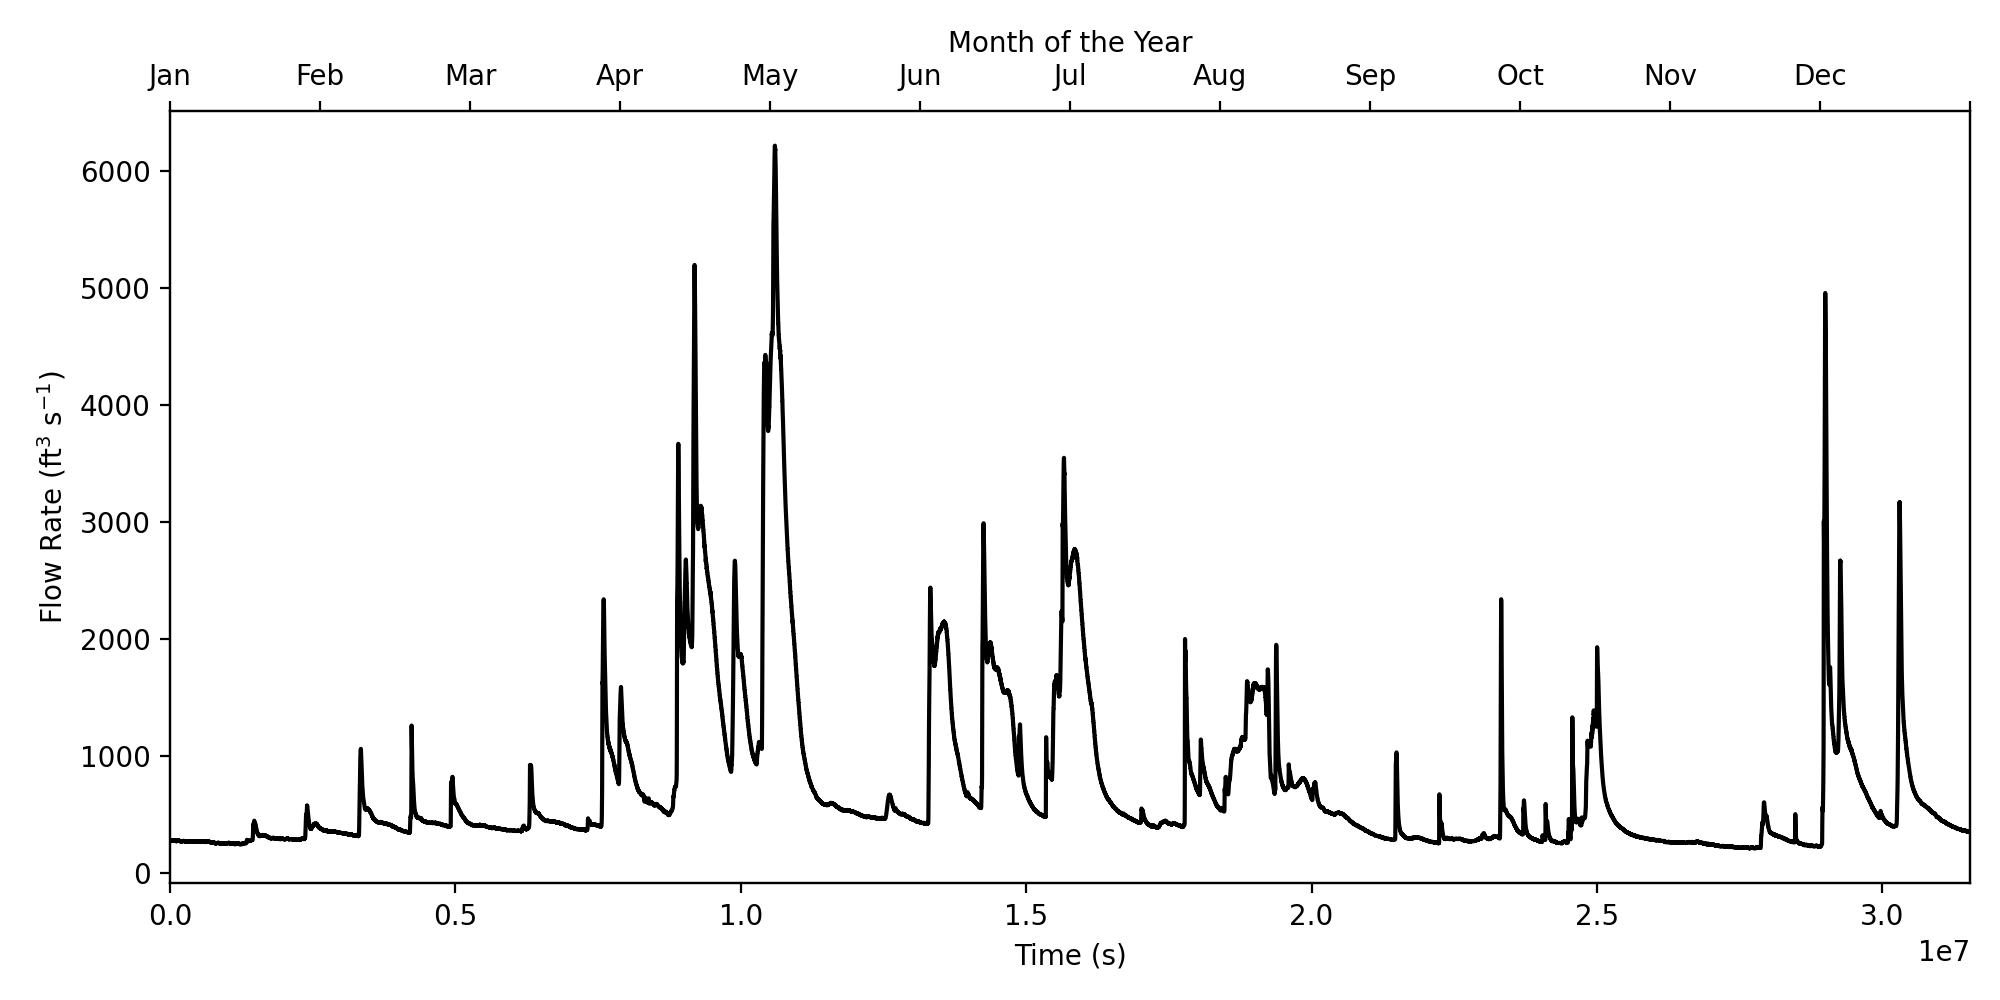
\includegraphics[width=1\linewidth]{Figures/2/dams.png}
    \caption{Flow-rate vs time along with the corresponding months for the year 2023}
    \label{dams}
\end{figure}

\subsection{Theoretical Approach}
Let $f(t)$ be the flow-rate of the dam as a function of time. To calculate the total water discharged in a time interval from $t_a$ to $t_b$, one can integrate $f(t)$ over that time.

\begin{align}
    \text{Water discharged } = \int_{t_a}^{t_b} f(t) dt
\end{align}

Let $W$ be the total water discharged in the year. Therefore,
\begin{align}
    W = \int_{0}^{T} f(t) dt
\end{align}

where $T$ is one year.

Our dataset consists of flow-rate of the dam at time stamps of 15 minutes. We have converted that to seconds to produce Fig. \ref{dams}. Since $f(t)$ is a collection of samples and not a well-defined function, we must perform numerical integration to find $W$.

% For simplicity, consider a small snippet of the above graph, which contains a sharp peak. Let us consider different ways of finding the flow rate in this particular time interval.

Let us discuss various ways of performing numerical integration of this discrete dataset.

\subsubsection{Mid-point Rule}
The mid-point rule algorithm divides the integral into equal sub-intervals and approximates the $f$ in each subinterval as $f(t)$. Then, it finds the area under the curve for each of those rectangular faces. This is one of the Newton-Cotes methods since it contains equally divided sub-intervals. 

If $h$ is the width of each sub-interval, the integral can be approximated as,

\begin{align}
    w = \int_{t_a}^{t_b} f(t) dt \approx h[f(\xi_0) + f(\xi_1) + ... + f(\xi_{n-1})]
\end{align}

where there are $n$ intervals and $\xi_i$ is the mid-point of $t_i$ and $t_{i+1}$.

We can use Taylor series expansion to find the error in the estimation. Consider a point $t_i$.

\begin{align}
    f(t) &= f(t_i) + (t-t_i)f'(\xi_i)\nonumber\\
    \int_{t_i}^{t_i+1} f(t)dt &= hf(t_i) + \frac{1}{2}h^2f'(\xi_i)\nonumber\,\,\, \left[\because h = t_{i+1}-t_i\right] \\
    \epsilon_i &= \frac{1}{2}h^2f'(\xi_i)
\end{align}

where $\epsilon_i$ is the absolute error in one single panel. For $n$ many panels, we can find the total error as a sum of error contributions of all the panels.

\begin{align}
    \epsilon &= \sum_{i=0}^{n-2} \frac{1}{2}h^2f'(\xi_i) =  \frac{n-1}{2}h^2f'(\xi_i) = \frac{t_b-t_a}{2}hf'(\xi_i)
\end{align}

\subsubsection{Trapezoidal Rule}
Another approximate method of calculating an integral is the trapezoidal (or trapezium) rule. Here, the area under the curve is approximated by a sum of $n$ trapezia instead of rectangles. 

For a single panel from $t_a$ to $t_b$,

\begin{align}
    \int_{t_a}^{t_b} f(t) dt \approx \frac{t_b-t_a}{2}(f(t_b)+f(t_a))
\end{align}

For $n$ many panels, 

\begin{align}
    \int_{t_a}^{t_b} f(t) dt \approx \frac{h}{2}(f(t_0)+2f(t_1)+2f(t_3)+...+2f(t_{n-1})+f(t_n))
\end{align}

All the points in the middle have double the weight because all of them get counted twice, once for the panel on the right and the other time for the panel on the left.

% the weight of the panels reflects the 
\subsubsection{Simpson's 1/3 Rule}
We have seen that the trapezoidal method approximates the integrand by a straight line. One could argue that a better approximation can be obtained by approximating the integrand with an easily integrable nonlinear function. Simpson's 1/3 rule uses quadratic interpolation of data to do the same.

Consider three points $t_1$, $t_2$ and $t_3$, through which we have to interpolate a quadratic polynomial $p(t)$. It follows that

\begin{align}
    p(t) = \alpha + \beta(t-t_1) + \gamma(t-t_1)(t-t_2)
\end{align}

where $\alpha, \beta$ and $\gamma$ are unknown constants evaluated from the such that polynomial passes through the points, $p(t_1) = f(t_1), p(t_2) = f(t_2)$ and $p(t_3) = f(t_3)$. These conditions yield

\begin{align}
    \alpha = f(t_1),\,\,\beta &=\frac{f(t_2)-f(t_1)}{(t_2-t_1)}\text{ and }\gamma = \frac{f(t_3)-2f(t_2)-f(t_1)}{(t_3-t_1)^2/2}\\
    \implies \int_{t_1}^{t_3} f(t)dt &\approx \int_{t_1}^{t_3} p(t)dt = \frac{(t_3-t_1)/2}{3}[f(t_1)+4f(t_2)+f(t_3)]\\
\end{align}

where $(t_3-t_1)/2 = h$. For a large number of panels, we can derive the composite Simpson's rule from the above equation as, 

\begin{align}
    \int_{t_a}^{t_b} f(t)dt \approx \frac{h}{3}\left[f(t_a)+4\sum_{i=2,4,6,..}^{n} f(t_i)+2\sum_{i=3,5,7,..}^{n-1} f(t_i)+f(t_b)\right]
\end{align}

where $(t_b-t_a)/n = h$, $n$ is the number of panels. The error in this estimation can be derived using Taylor series expansion as,

\begin{align}
    \epsilon_i = \frac{-1}{90}h^5f^{4}(\xi_i) \implies \epsilon = \frac{-(t_b-t_a)}{180}h^4f^{4}(\xi)
\end{align}

\subsubsection{Simpson's 3/8 Rule}
This method uses cubic interpolation of data points to approximate the integrand. Since a third-order polynomial can be only determined from four points (i.e. three panels), the total integral for 1 panel is approximated to,

\begin{align}
    \int_{t_1}^{t_3} f(t)dt \approx \int_{t_1}^{t_3} p(t)dt = \frac{3(t_2-t_1)}{8}[f(t_1)+3f(t_2)+3f(t_3)+f(t_4)]
\end{align}

Where the name 3/8 method comes from the 3/8 factor in the expression. For a large number of panels, we can derive composite Simpson's 3/8 rule as,

\begin{align}
    \int_{t_a}^{t_b} f(t)dt \approx \frac{3h}{8}\left[f(t_a)+3\sum_{i=2,5,8,..}^{n-1} (f(t_i)+f(t_{i+1})+2\sum_{i=4,7,10,..}^{n-2} f(t_i)+f(t_b)\right]
\end{align}

where the interval is divided into $n$ subintervals and $n$ is a multiple of 3. $h$ is the fixed time interval between two data points.

The error in this estimation can be derived using Taylor series expansion  (\cite{matthews-2004}),

\begin{align}
    \epsilon_i = \frac{-3}{80}h^5f^{4}(\xi_i) \implies \epsilon = \frac{-(t_b-t_a)}{80}h^4f^{4}(\xi)
\end{align}

\subsection{Implementation and results}
Before finding the total annual water discharge, let us first consider a small snippet of our data with a significantly sharp peak. We will first try to find the area under the curve in this domain.

\begin{figure}[H]
    \centering
    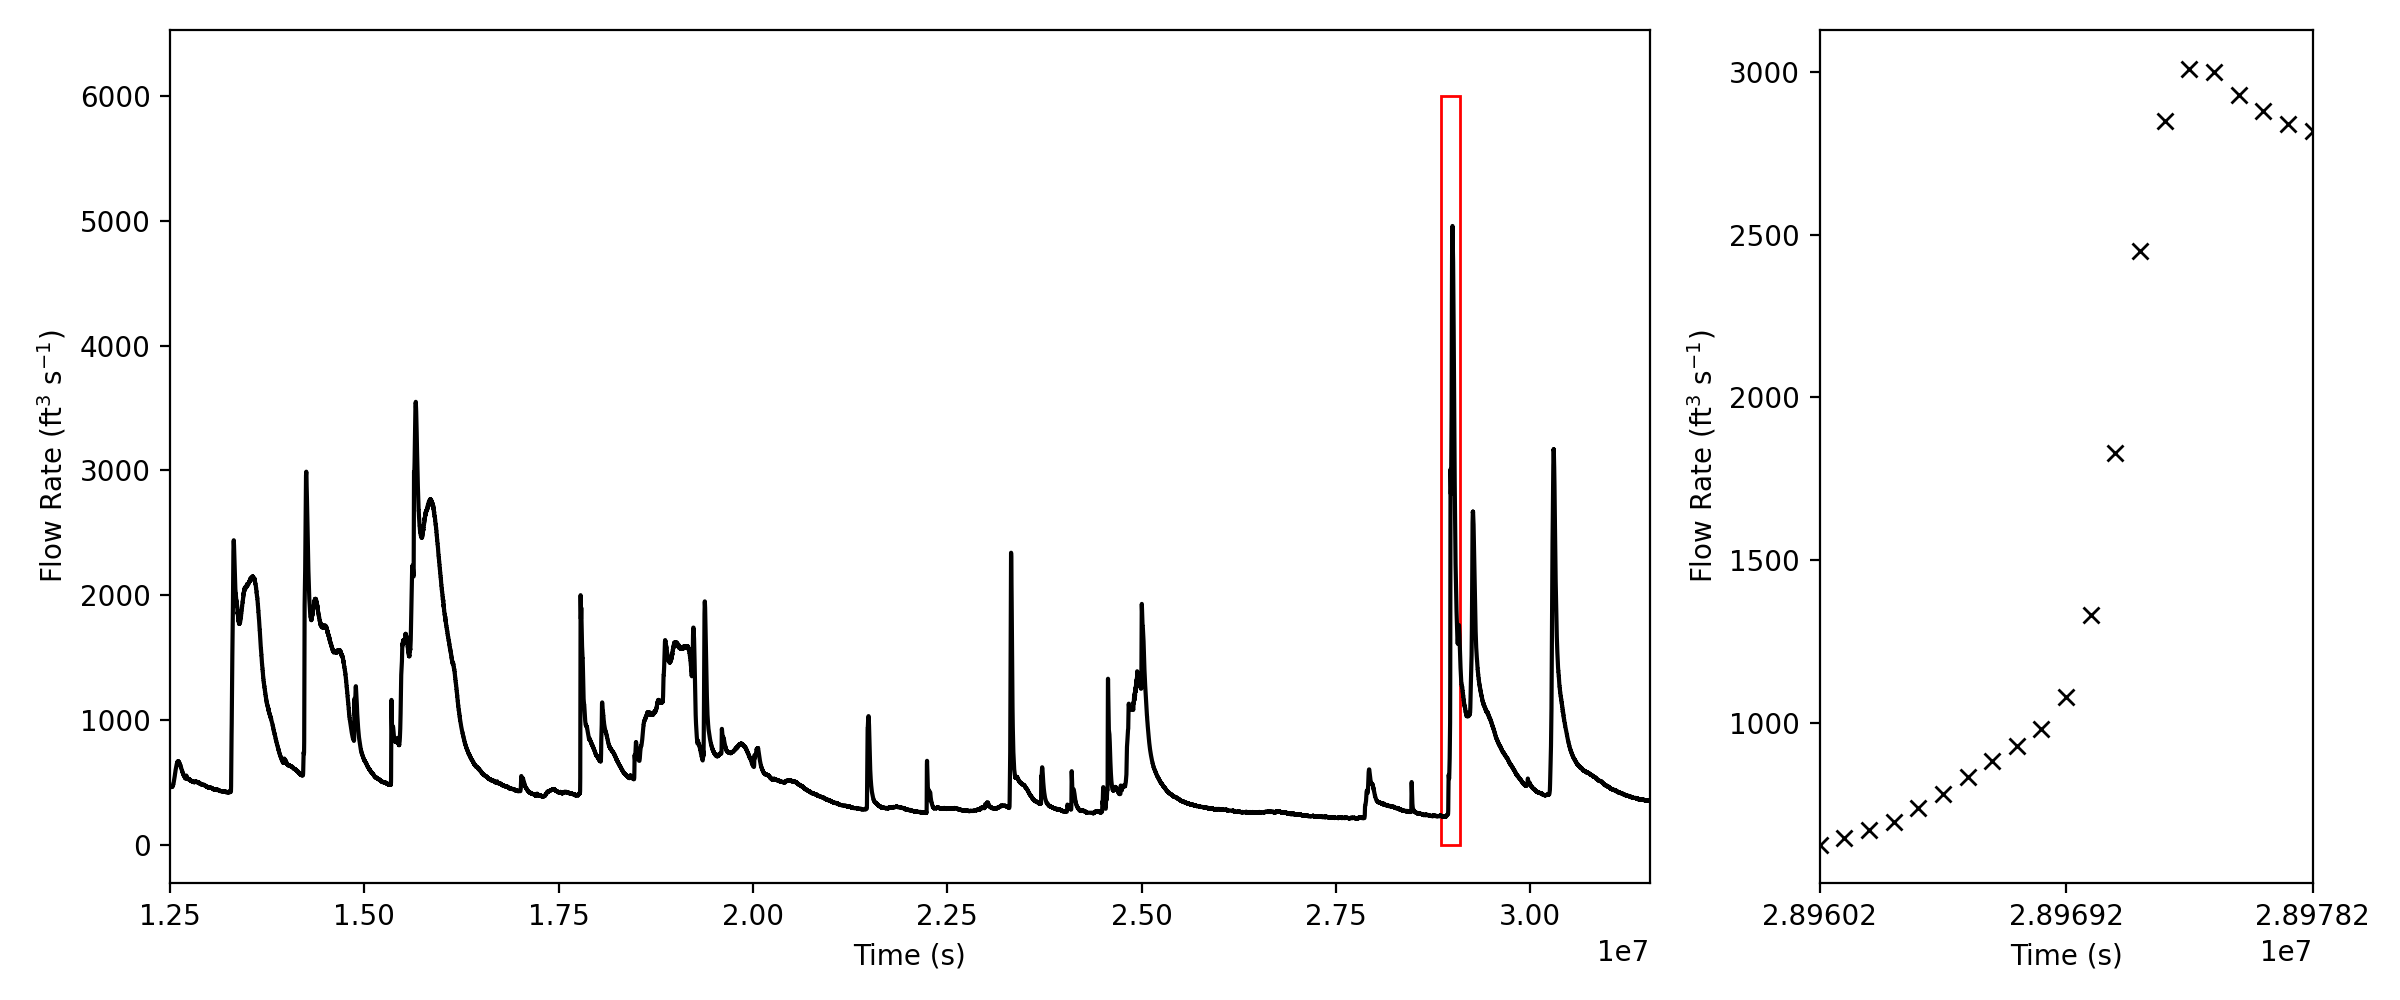
\includegraphics[width=1\linewidth]{Figures/2/zoom.png}
    \caption{The right panel shows the zoomed-up version of the highlighted section with a very sharp peak we will be focusing on}
\end{figure}

Here we have found this particular region of interest using 
\begin{lstlisting}[language=Python, caption=Isolating the region of interest]
roi = np.where((t>2.896e7) & (t<2.898e7))
f1 = flow[roi]
t1 = t[roi]
t1 = (t1-np.min(t1)) # changing the range of x from 0 to 1 for simplicity
t1 = t1/np.max(t1)
dx = t1[1]-t1[0]
\end{lstlisting}

We have implemented the discussed integration methods in the following code snippet.

\begin{lstlisting}[language=Python, caption=Code implementing different integration techniques and their associated errors]
    import numpy as np
    import matplotlib.pyplot as plt
    from datetime import datetime
    from scipy.interpolate import interp1d
    
    """ Extract flow-rate information from the csv file"""
    dates, times, flow = np.loadtxt('project/data/water.csv', unpack = True, usecols = (2, 3, 5), dtype=object)
    flow = np.array(flow, dtype=float)
    t = np.zeros(dates.size)
    for i in range(dates.size):
        d = datetime.strptime(dates[i]+times[i], '%Y-%m-%d%H:%M')
        t[i] = d.timestamp()
    start_time = t[0]
    t -= start_time
    
    """ Calculate derivatives using central difference approach 
    used in the calculation of error"""
    def d2dt(y,h=1):
        diffs = np.zeros(len(y))
        for x in range(2, len(y)-2):
            diffs[x] = (y[x+1]+y[x-1]-2*y[x])/(h**2)
        return diffs
    
    def d4dt(y,h=1):
        diffs = np.zeros(len(y))
        for x in range(2, len(y)-2):
            diffs[x] = (y[x+2]-4*y[x+1]+6*y[x]-4*y[x-1]+y[x-2])/h**4
        return diffs
    
    """ Integration functions """
    def mid_point_integration(x, y):
        half_step = (x[1]-x[0])/2
        res = 0
        res += y[0]*half_step
        for i in range(1,len(x)-1):
            res += y[i]*half_step*2
        res += y[-1]*half_step
    
        f2epsilon = np.max(abs(d2dt(y)))
        err = ((x[-1]-x[0]) * f2epsilon * dx**2)/(24)
        return res, err
    
    def trapezoidal_integration(x, y, dx):
        res = (dx/2) * (y[0] + 2*np.sum(y[1:-1]) + y[-1])
        f2epsilon = np.max(abs(d2dt(y)))
        err = ((x[-1]-x[0]) * f2epsilon * dx**2)/(12)
        return res, err
    
    def simpsons_13_integration(x, y, dx):
        # If there are an even number of samples, N, then there are an odd
        # number of intervals (N-1), but Simpson's rule requires an even number
        # of intervals. Hence we perform simpson's rule on the first and last (N-2)
        # intervals, take the average and add up the end points using trapezoidal rule
        if len(x) % 2 == 0:
            res = (dx/3) * (y[0] + 4*np.sum(y[1:-2:2]) + 2*np.sum(y[2:-2:2]) + y[-3])
            res += (dx/3) * (y[1] + 4*np.sum(y[2:-1:2]) + 2*np.sum(y[3:-1:2]) + y[-2])
            res /= 2
            res += 0.5*dx*(y[0] + y[-1])
        else:
            res = (dx/3) * (y[0] + 4*np.sum(y[1:-1:2]) + 2*np.sum(y[2:-1:2]) + y[-1])
        f4epsilon = np.max(abs(d4dt(y)))
        err = ((x[-1]-x[0]) * f4epsilon * (dx**4))/(180)
        return res, err
    
    def simpsons_38_integration(x, y, dx):
        # If there are an N number of samples, then there are an (N-1)
        # number of intervals. Simpson's 3/8 rule requires an 3n number
        # of intervals. Hence in case of 3n-1 or 3n-2 intervals, we approximate the end points
        # similar to what we did for Simpson's 1/3 rule
        if len(x) % 3 == 0: # (n-1)%3 = 2
            res = y[0] + 3*(np.sum(y[1:-3:3])+np.sum(y[2:-3:3])) + 2*np.sum(y[3:-3:3])+ y[-3]
            res += y[1] + 3*(np.sum(y[2:-2:3])+np.sum(y[3:-2:3])) + 2*np.sum(y[4:-2:3])+ y[-2]
            res += y[2] + 3*(np.sum(y[3:-1:3])+np.sum(y[4:-1:3])) + 2*np.sum(y[5:-1:3])+ y[-1]
            res *= (3*dx/8) * (1/3)
            res += dx*(y[0] + y[-1])
        elif len(x) % 3 == 1: # (n-1)%3 = 0
            res = y[0] + 3*(np.sum(y[1:-1:3])+np.sum(y[2:-1:3])) + 2*np.sum(y[3:-1:3])+ y[-1]
            res *= (3*dx/8)
        elif len(x) % 3 == 2: #(n-1)%3 = 1
            res = y[0] + 3*(np.sum(y[1:-2:3])+np.sum(y[2:-2:3])) + 2*np.sum(y[3:-2:3])+ y[-2]
            res += y[1] + 3*(np.sum(y[2:-1:3])+np.sum(y[3:-1:3])) + 2*np.sum(y[4:-1:3])+ y[-1]
            res *= (3*dx/8) * (1/2)
            res += 0.5*dx*(y[0] + y[-1])
    
        f4epsilon = np.max(abs(d4dt(y)))
        err = ((x[-1]-x[0]) * f4epsilon * (dx**4))/(80)
        return res, err
    
    """ Convert the domain to [0, 1] for simplicity in calculation of errors 
    and then multiply by t_final (t_inital = 0)"""
    tmax = t[-1]-t[0]
    int_t = t/np.max(t)
    dx = int_t[1]-int_t[0]
    
    mid_point, max_error_mid_point = mid_point_integration(int_t, flow)
    trapezoidal, max_error_trapz = trapezoidal_integration(int_t, flow, dx)
    simpsons_13, max_error_simpsons13 = simpsons_13_integration(int_t, flow, dx)
    simpsons_38, max_error_simpsons38 = simpsons_38_integration(int_t, flow, dx)
    
    """ Multipy the integrand values by tmax and the error values by tmax*(dt)^2 and tmax*(dt)^4 for different integration methods
    as required. Here, since our data points are 15 minutes apart, dt is taken to be 900 seconds."""
    print(f'Mid-point: {mid_point*tmax*1e-9:.3f} x 10^9 \pm {max_error_mid_point*tmax*(900**2)*1e-5:.3f} x 10^5 ft^3')
    print(f'Trapezoidal: {trapezoidal*tmax*1e-9:.3f} x 10^9 \pm {max_error_trapz*tmax*(900**2)*1e-5:.3f} x 10^5 ft^3')
    print(f'Simpsons 1/3: {simpsons_13*tmax*1e-9:.3f} x 10^9 \pm {max_error_simpsons13*tmax*(900**4):.3f} ft^3')
    print(f'Simpsons 3/8: {simpsons_38*tmax*1e-9:.3f} x 10^9 \pm {max_error_simpsons38*tmax*(900**4):.3f} ft^3')
\end{lstlisting}

Now, running our program on the region of interest, we can test the effectiveness of our code especially while integrating sharp features.

\begin{figure}[H]
     \centering
     \begin{subfigure}[b]{0.45\textwidth}
         \centering
         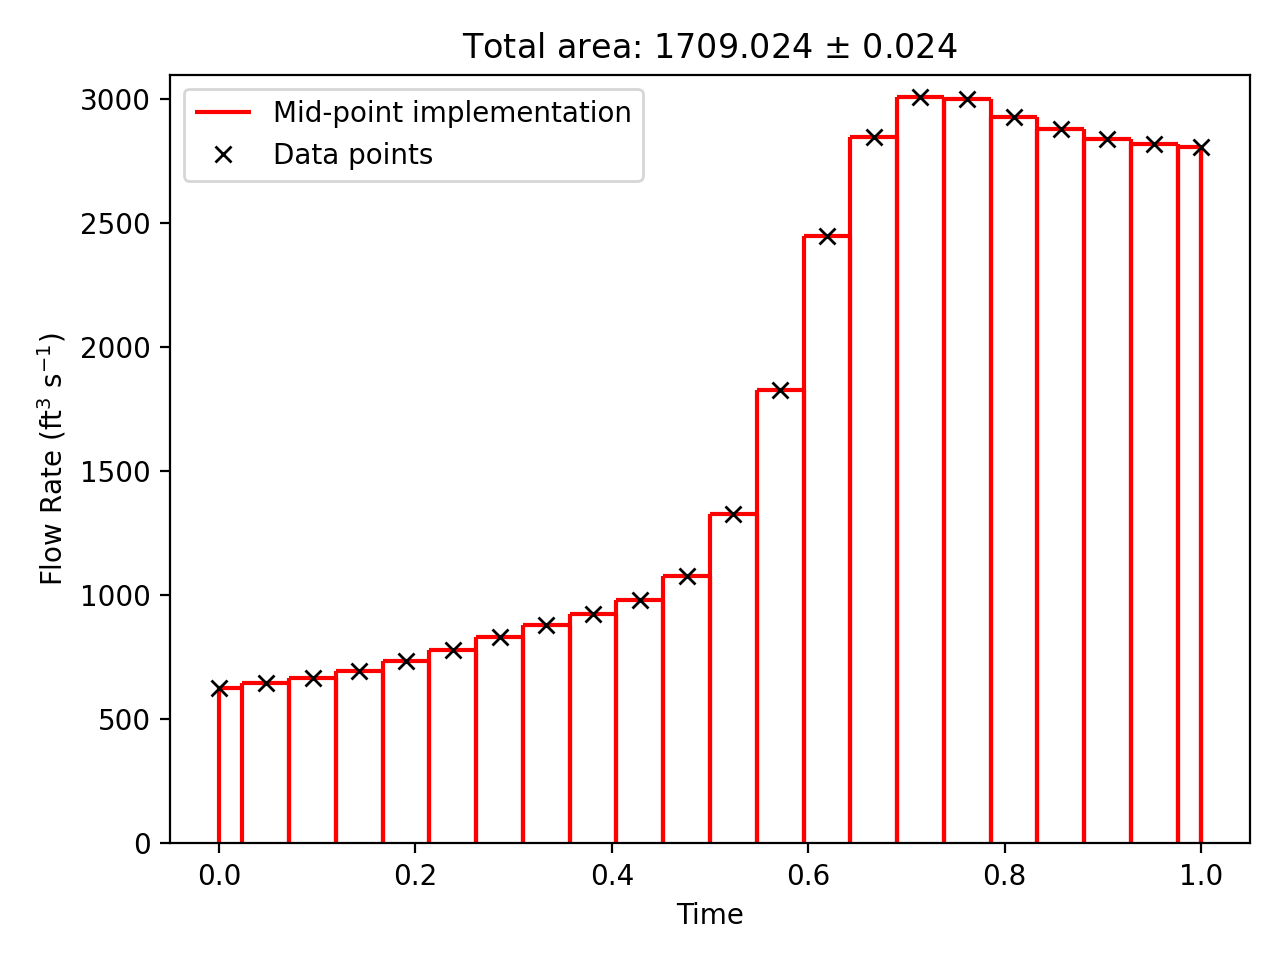
\includegraphics[width=\textwidth]{Figures/2/mid-point.png}
         \caption{Mid-Point Method}
     \end{subfigure}
     \begin{subfigure}[b]{0.45\textwidth}
         \centering
         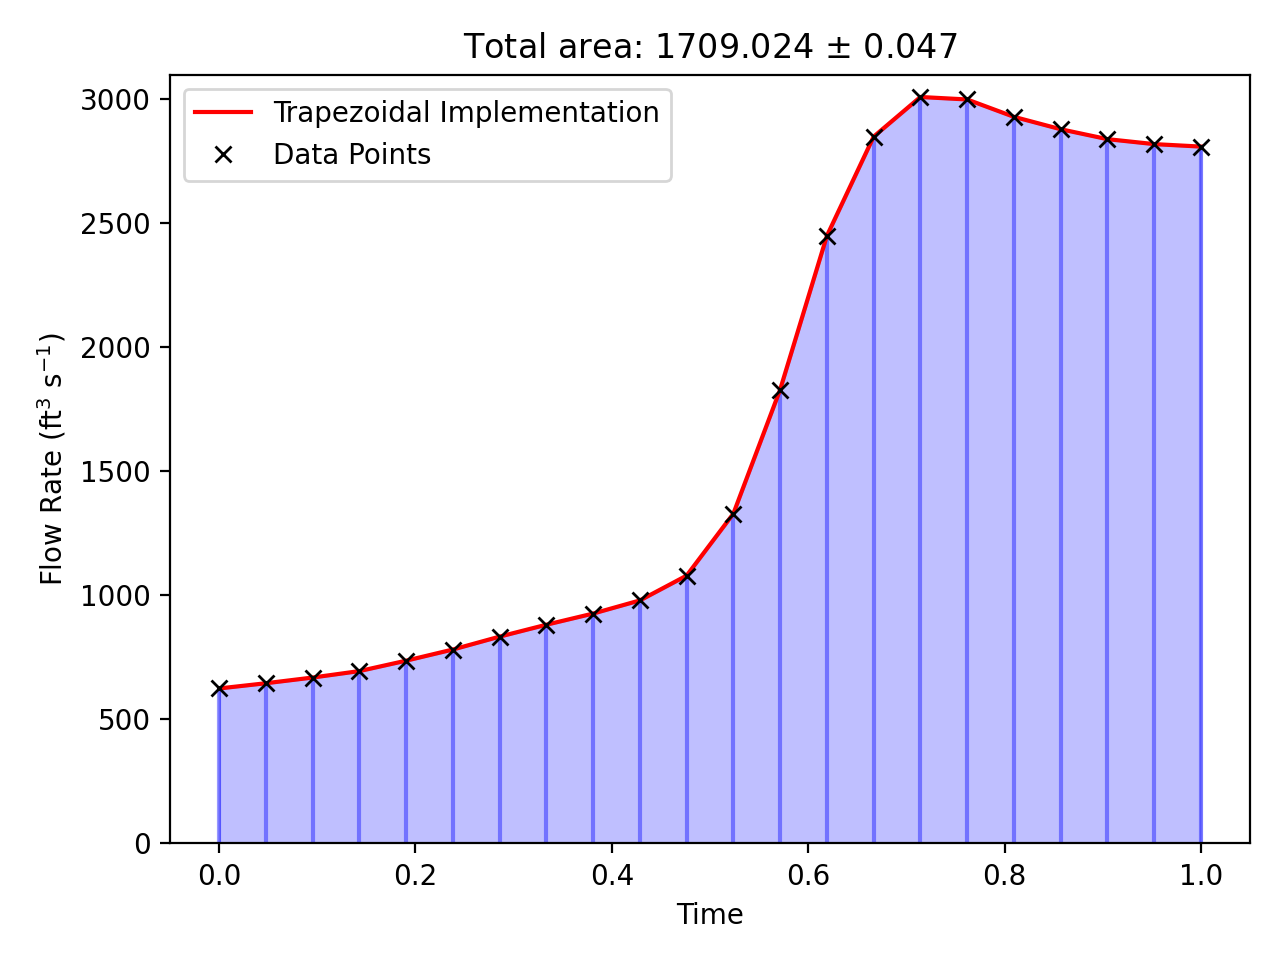
\includegraphics[width=\textwidth]{Figures/2/trapezoidal.png}
         \caption{Trapezoidal Method}
     \end{subfigure}
     \begin{subfigure}[b]{0.45\textwidth}
         \centering
         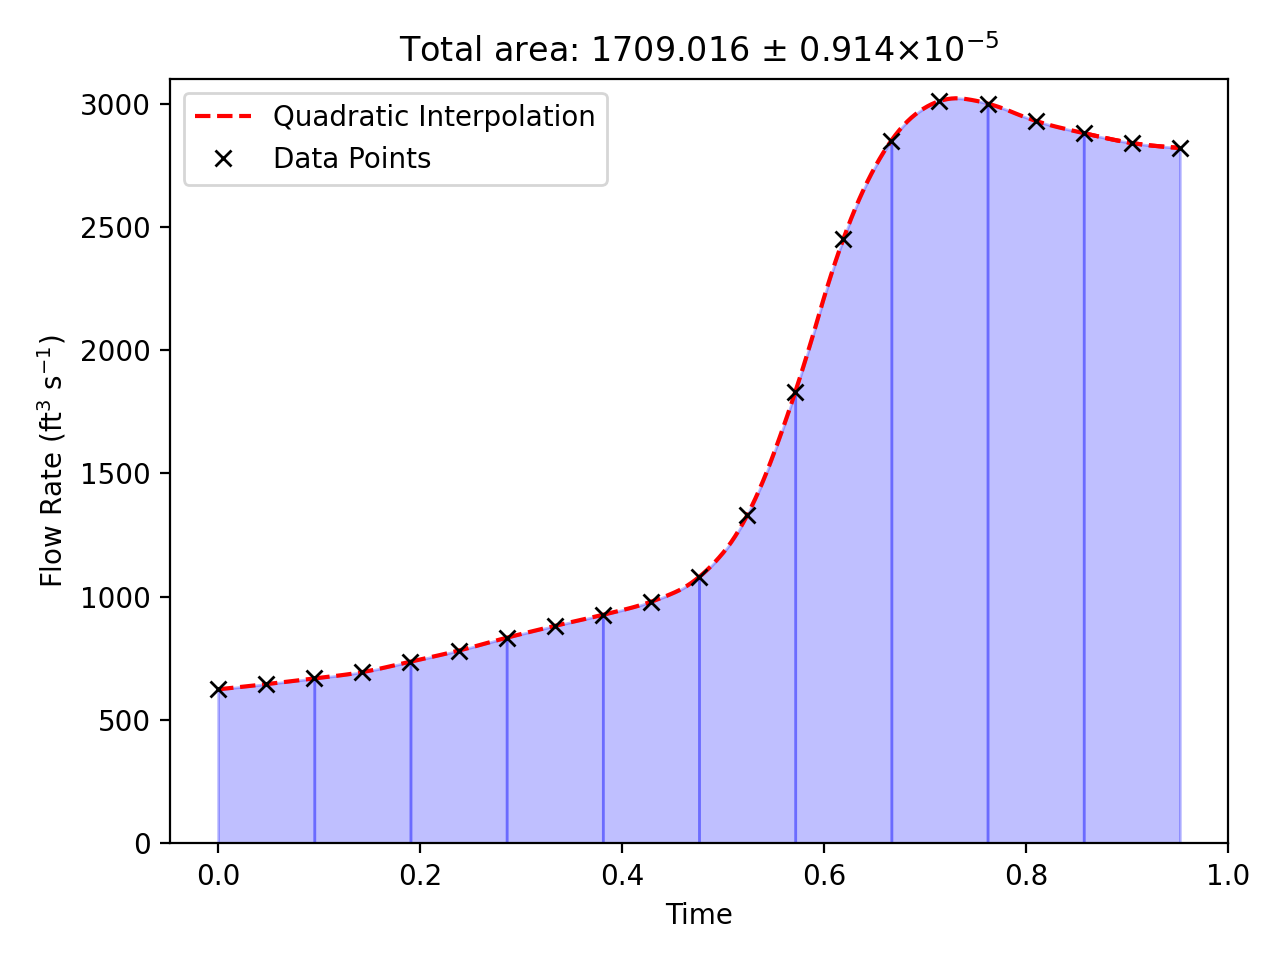
\includegraphics[width=\textwidth]{Figures/2/simpsons13.png}
         \caption{Simpson's 1/3 rule with quadratic interpolation}
     \end{subfigure}
     \begin{subfigure}[b]{0.45\textwidth}
         \centering
         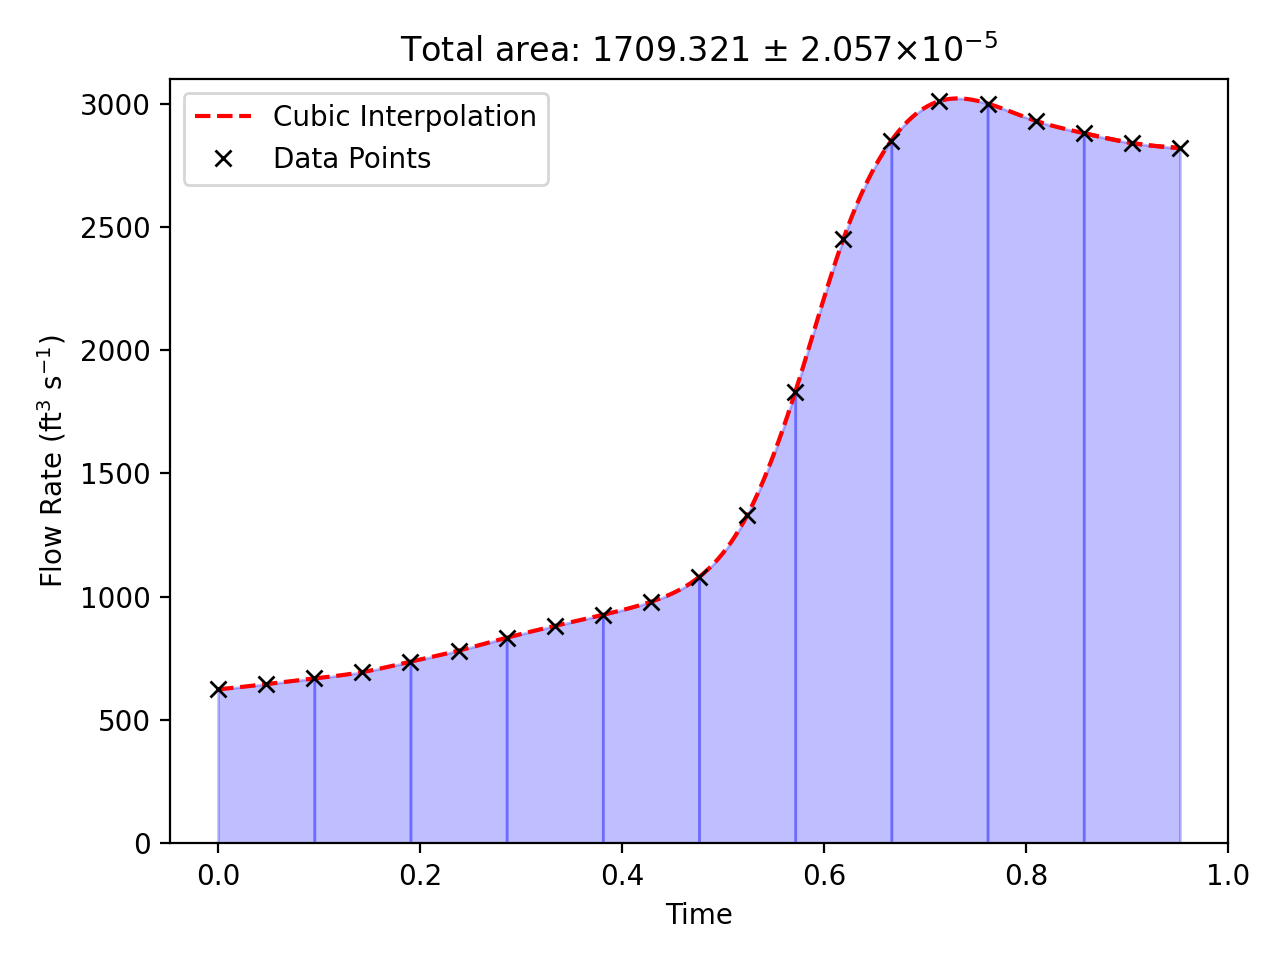
\includegraphics[width=\textwidth]{Figures/2/simpsons38.png}
         \caption{Simpson's 3/8 rule with cubic interpolation}
     \end{subfigure}
    \caption{All mentioned integration techniques implemented for the small snippet with 22 data points.}
\end{figure}

\subsection{Discussion}
We have employed 4 different methods to calculate the total water discharged annually. The results obtained are:

\begin{align*}
    \text{Using Mid-point method,  } W &= (23.207 \times 10^{9} \pm 2.167 \times 10^5) \text{ ft}^3\\
    \text{Using Trapezoidal Rule,  } W &= (23.207 \times 10^{9} \pm 4.337 \times 10^5) \text{ ft}^3\\
    \text{Using Simpson's 1/3 Rule,  } W &= (23.207 \times 10^{9} \pm 24.405) \text{ ft}^3\\
    \text{Using Simpson's 3/8 Rule,  } W &= (23.207 \times 10^{9} \pm 54.910) \text{ ft}^3
\end{align*}

\noindent As we can see, the values obtained using different match quite well with each other, with varying levels of accuracy.
Hence, we can say that our result is quite precise.

Since our flow-rate function is not a well-defined function, we cannot use methods like Gaussian or Lagrange quadrature, which are generally more precise. Here our abscissas are predetermined; hence, we can only use one of the Newton-Cotes methods.